\documentclass{rs}
\usepackage{amsmath,amssymb,amsthm,stmaryrd}
\usepackage[all]{xy}
\usepackage[usenames,dvipsnames]{xcolor}
\usepackage{tikz}
\usepackage{url}
\usepackage{hyperref}
\usepackage{enumerate}
\usepackage{tensor}
%/home/grad/zyf/TeX/inputs/
\usepackage{mathrsfs}
\usepackage{graphicx}
\usepackage{mathtools}
\usetikzlibrary{arrows}
%\usepackage{amsrefs}
%\usepackage{setspace}
%\doublespacing
\usepackage{ulem}

%\title{Elliptic curves}
%\author{Yifei Zhu}
%\givenname{Yifei}
%\surname{Zhu}
%\address{Department of Mathematics\\University of Minnesota\\Minneapolis, MN 55455\\USA}
%\email{zyf@math.umn.edu}

%\subject{primary}{msc2000}{55P99}
%\subject{secondary}{msc2000}{55Q99}

%\bibliographystyle{gtart}
\parskip 0.7pc
\parindent 0pt

\newtheorem{thm}[equation]{Theorem}
\newtheorem{cor}[equation]{Corollary}
\newtheorem{prop}[equation]{Proposition}
\newtheorem{lem}[equation]{Lemma}
\theoremstyle{definition}
\newtheorem{defn}[equation]{Definition}
\newtheorem{cstr}[equation]{Construction}
\theoremstyle{remark}
\newtheorem{rmk}[equation]{Remark}
\newtheorem{ex}[equation]{Example}
\newtheorem{case}[equation]{Case}
\newtheorem{slogan}[equation]{Slogan}
\newtheorem{ques}[equation]{Question}

\def\co{\colon\thinspace}
\newcommand{\mb}[1]{\mathbb{#1}}
\newcommand{\mf}[1]{\mathfrak{#1}}
\newcommand{\Hom}{\ensuremath{{\rm Hom}}}
\newcommand{\Aut}{{\rm Aut}}
\newcommand{\LT}{{\rm LT}}
\newcommand{\Spec}{{\rm Spec\thinspace}}
\newcommand{\Proj}{{\rm Proj\thinspace}}
\newcommand{\Spf}{{\rm Spf\thinspace}}
\newcommand{\Ell}{{\rm Ell}}
\newcommand{\Sch}{{\rm Sch}}
\newcommand{\cF}{\overline {\mb F}}
\newcommand{\ck}{\overline k}
\newcommand{\CA}{{\cal A}}
\newcommand{\CB}{{\cal B}}
\newcommand{\CC}{{\cal C}}
\newcommand{\CE}{{\cal E}}
\newcommand{\CF}{{\cal F}}
\newcommand{\CG}{{\cal G}}
\newcommand{\CH}{{\cal H}}
\newcommand{\CHom}{{\cal H}om}
\newcommand{\CLie}{{\cal L}ie}
\newcommand{\CM}{{\cal M}}
\newcommand{\CO}{{\cal O}}
\newcommand{\CP}{{\cal P}}
\newcommand{\CS}{{\cal S}}
\newcommand{\Mod}{{\rm Mod}}
\newcommand{\Alg}{{\rm Alg}}
\newcommand{\dl}{{\rm DL}}
\newcommand{\Set}{{\rm Set}}
\newcommand{\Sq}{{\rm Sq}}
\newcommand{\Sub}{{\rm Sub}}
\newcommand{\Frob}{{\rm Frob}}
\renewcommand{\gcd}{{\rm gcd}}
\newcommand{\cmp}{{\rm cmp}}
\newcommand{\DF}{{{\rm DefFrob}_\BG}}
\newcommand{\Model}{{\rm Model}}
\newcommand{\HGa}{{\widehat{\mb G}_a}}
\newcommand{\HGm}{{\widehat{\mb G}_m}}
\newcommand{\Gm}{{{\mb G}_m}}
\newcommand{\DL}{Dyer-Lashof~}
\newcommand{\EM}{Eilenberg-Mac~Lane~}
\newcommand{\BC}{{\mb C}}
\newcommand{\BE}{{\mb E}}
\newcommand{\BF}{{\mb F}}
\newcommand{\BG}{{\mb G}}
\newcommand{\BN}{{\mb N}}
\newcommand{\BP}{{\mb P}}
\newcommand{\BQ}{{\mb Q}}
\newcommand{\BR}{{\mb R}}
\newcommand{\BW}{{\mb W}}
\newcommand{\BZ}{{\mb Z}}
\newcommand{\fm}{{\mf m}}
\newcommand{\HC}{\widehat{C~}\!}
\newcommand{\HE}{\widehat{E~}\!}
\newcommand{\Hf}{\widehat{f}}
\newcommand{\Hphi}{\widehat{\phi}}
\newcommand{\Hpsi}{\widehat{\psi}}
\newcommand{\HS}{\widehat{S~}\!}
\newcommand{\TA}{\tilde{\A}}
\newcommand{\Tc}{\tilde{c}}
\newcommand{\TE}{\widetilde{E\thinspace}\!}
\newcommand{\Tf}{\widetilde{f}}
\newcommand{\Tp}{\widetilde{\psi}}
\newcommand{\TW}{\widetilde{W\thinspace}\!}
\newcommand{\md}{~~{\rm mod}~}
\newcommand{\ad}{{\rm and}}
\newcommand{\DR}{{\scriptscriptstyle \rm DR}}
\newcommand{\HT}{{\rm ht}}
\newcommand{\id}{{\rm id}}
\newcommand{\op}{{\rm op}}
\newcommand{\tf}{{\rm tf}}
\newcommand{\TMF}{{\rm TMF}}
\newcommand{\MF}{{\rm MF}}
\newcommand{\tr}{{\rm trace}}
\newcommand{\univ}{{\rm univ}}
\newcommand{\Ext}{{\rm Ext}}
\newcommand{\Tor}{{\rm Tor}}
\newcommand{\nul}{{\rm nul}}
\newcommand{\A}{\alpha}
\newcommand{\B}{\beta}
\renewcommand{\D}{\Delta}
\renewcommand{\d}{\delta}
\newcommand{\f}{\phi}
\newcommand{\G}{\Gamma}
\newcommand{\g}{\gamma}
\newcommand{\K}{\kappa}
\renewcommand{\l}{\lambda}
\newcommand{\si}{\sigma}
\newcommand{\T}{\tau}
\newcommand{\om}{\underline{\omega\!}_{~E/S}}
\newcommand{\p}{\psi^3}
\newcommand{\s}{S^\bullet}
\newcommand{\ce}{\coloneqq}
\newcommand{\lb}{\llbracket}
\newcommand{\rb}{\rrbracket}
\newcommand{\lp}{(\!(}
\newcommand{\rp}{)\!)}
\newcommand{\Ht}{\widehat{T}}
\newcommand{\Tt}{\widetilde{T}}
\newcommand{\mt}{\widetilde{m}}
\newcommand{\lt}{\widetilde{\lambda}}
\newcommand{\todo}{\spadesuit}
\newcommand{\totodo}{\heartsuit}
\renewcommand{\=}{\approx}
\renewcommand{\-}{\sim}
\newcommand{\isog}[1]{Proposition \ref{prop:isog}\thinspace \eqref{isog(#1)}}
\newcommand{\q}[1]{Proposition \ref{prop:Q}\thinspace \eqref{Q(#1)}}
\newcommand{\go}[1]{Definition \ref{def:go}\thinspace \eqref{go(#1)}}
\newcommand{\rd}[1]{{\textcolor{red}{#1}}}
\newcommand{\bl}[1]{{\textcolor{blue}{#1}}}
\newcommand{\wt}[1]{\textcolor{white}{#1} \!~}
\newcommand{\GL}{{\rm GL}}
\newcommand{\SL}{{\rm SL}}
\newcommand{\Tate}{{\rm Tate}}
\renewcommand{\c}[2]{{#1 \choose #2}}

\makeatletter
\DeclareRobustCommand\widecheck[1]{{\mathpalette\@widecheck{#1}}}
\def\@widecheck#1#2{%
    \setbox\z@\hbox{\m@th$#1#2$}%
    \setbox\tw@\hbox{\m@th$#1%
       \widehat{%
          \vrule\@width\z@\@height\ht\z@
          \vrule\@height\z@\@width\wd\z@}$}%
    \dp\tw@-\ht\z@
    \@tempdima\ht\z@ \advance\@tempdima2\ht\tw@ \divide\@tempdima\thr@@
    \setbox\tw@\hbox{%
       \raise\@tempdima\hbox{\scalebox{1}[-1]{\lower\@tempdima\box
\tw@}}}%
    {\ooalign{\box\tw@ \cr \box\z@}}}
\makeatother

\numberwithin{equation}{section}
\renewcommand{\theequation}{\thesection.\arabic{equation}}



\begin{document}
\section{Canonical modular polynomials}
\label{sec:cmp}

\begin{center}
 \includegraphics[scale=.23]{ssing} \\
 {\small \cite[Section VI.6]{DR}} 
\end{center}

Using Magma's \href{http://magma.maths.usyd.edu.au/calc}{calculator}, 
we reproduce the first few {\em canonical modular polynomials} from its 
\href{http://magma.maths.usyd.edu.au/magma/handbook/modular_curves}{Modular Polynomial Databases}.\footnote{available up to $\G_0(127)$}  
We note the following, to return to.  

\begin{enumerate}[(i)]
 \item \rd{Difference from $j = 744$ equals $\#\Aut(E_\text{s.s.}/\cF_p)$.}  

 \item Constant term equals $p^s$ where $s = 12 / \gcd(p - 1, 12) \stackrel{?}{=} \prod \big(\#\Aut(E_\text{s.s.}/\cF_p)/2\big)$.  

 \item Linear coefficient reduces to supersingular $j$-invariants in the diagram above.  (What is the pattern for their exponents?)  
\end{enumerate}

\begin{itemize}
 \item $g = 0$ 
 \[
  \begin{split}
    \G_0(2) \qquad & ~ x^3+48 x^2+(\rd{768-j}) x+2^{12} \\
            \equiv & ~ x (x^2 - j) \md 2 \\
    \G_0(3) \qquad & ~ x^4+36 x^3+270 x^2+(\rd{756-j}) x+3^6 \\
            \equiv & ~ x (x^3 - j) \md 3 \\
    \G_0(5) \qquad & ~ x^6+30 x^5+315 x^4+1300 x^3+1575 x^2+(\rd{750-j}) x+5^3 \\
            \equiv & ~ x (x^5 - j) \md 5 \\
    \G_0(7) \qquad & ~ x^8+28 x^7+322 x^6+1904 x^5+5915 x^4+8624 x^3+4018 x^2+(\rd{748-j}) x+7^2 \\
            \equiv & ~ x \big(x^7 - (j - 1728)\big) \md 7 \\
   \G_0(13) \qquad & ~ x^{14}+26 x^{13}+325 x^{12}+2548 x^{11}+13832 x^{10}+54340 x^9+157118 x^8 \\
                   & +333580 x^7+509366 x^6+534820 x^5+354536 x^4+124852 x^3+15145 x^2 \\
                   & +(\rd{746-j}) x+13^1 \\
            \equiv & ~ x \big(x^{13} - (j - 5)\big) \md 13 
  \end{split}
 \]

 \item $g = 1$ 
 \[
  \begin{split}
   \G_0(11) \qquad & ~ x^{12}-5940 x^{11}+14701434 x^{10}+(-139755 j-19264518900) x^9 \hskip 2.2cm \\
                   & +(723797800 j +13849401061815) x^8+(67496 j^2-1327909897380 j \\
                   & -4875351166521000) x^7+(2291468355 j^2+1036871615940600 j \\
                   & +400050977713074380) x^6+(-5346 j^3+4231762569540 j^2 \\
                   & -310557763459301490 j+122471154456433615800) x^5+(161201040 j^3 \\
                   & +755793774757450 j^2+17309546645642506200 j \\
                   & +6513391734069824031615) x^4+(132 j^4-49836805205 j^3 \\
                   & +6941543075967060 j^2-64815179429761398660 j \\
                   & +104264884483130180036700) x^3+(468754 j^4+51801406800 j^3 \\
                   & +214437541826475 j^2+77380735840203400 j+804140494949359194) x^2 \\
                   & +(-j^5+3732 j^4-4586706 j^3+2059075976 j^2-253478654715 j \\
                   & +2067305393340) x+11^6 \\
            \equiv & ~ x \big(x^{11} - j^2 (j - 1728)^3\big) \md 11 \\
   \G_0(17) \qquad & ~ x^{18}+510 x^{17}+125001 x^{16}+19248080 x^{15}+2058738420 x^{14} \\
                   & +(10846 j +160172066760) x^{13}+(6027384 j+9242645403716) x^{12} \\
                   & + \cdots \\
                   & +(-j^4+2982 j^3-2547081 j^2 +567877726 j-8730057090) x+17^3 \\
            \equiv & ~ x \big(x^{17} - j (j - 8)^3\big) \md 17 \\
   \G_0(19) \qquad & ~ x^{20}-152 x^{19}+11020 x^{18}-509732 x^{17}+16884502 x^{16}-423717176 x^{15} \\
                   & +8284685786 x^{14}+(-950 j-127757600560) x^{13} \\
                   & + \cdots \\
                   & +(-j^3+2236 j^2-1075910 j +37507528) x+19^2 \\
            \equiv & ~ x \big(x^{19} - (j - 7) (j - 1728)^2\big) \md 19 
  \end{split}
 \]

 \item $g > 1$ 
 \[
  \begin{split}
   \G_0(23) \qquad & ~ x^{24} + 94392 x^{23} + 4240527204 x^{22} + (108774498 j + 119018915927208) x^{21} \hskip .4cm \\
                   & + \cdots \\
                   & +(-j^{11} + 8196 j^{10} - 28368090 j^9 + 53962467848 j^8 - 61514962720527 j^7 \\
                   & + 43007336651707740 j^6 - 18144237478297458590 j^5 \\
                   & + 4374793948754527714200 j^4 - 541459535600500383823479 j^3 \\
                   & + 28035152457942175237515676 j^2 - 389561380516779182551042062 j \\
                   & + 312190445452533657242901912) x + 23^6 \\
            \equiv & ~ x \big(x^{23} - j^2 (j + 4)^6 (j - 1728)^3\big) \md 23 \\
  \end{split}
 \]
 \[
  \begin{split}
   \G_0(29) \qquad & ~ x^{30} - 1218 x^{29} + 750375 x^{28} - 312177460 x^{27} + 97844061669 x^{26} \\
   \hskip 2.4cm      & + (-236321 j - 24383203360230) x^{25} +(946283688 j + 4982726503407419) x^{24} \\
                   & + \cdots \\
                   & +(-j^7 + 5214 j^6 - 10272861 j^5 + 9480438286 j^4 - 4108842162480 j^3 \\
                   & + 728011816505784 j^2 - 35575638370254161 j + 107281337499515022) x + 29^3 \\
            \equiv & ~ x \big(x^{29} - j (j - 2)^3 (j + 4)^3\big) \md 29 
  \end{split}
 \]
\end{itemize}

We compare these to modular equations for $\big(\G_0(p),\G_1(N)\big)$ computed previously.  

\begin{itemize}
 \item $g = 0$\footnote{\cite[Theorem 10.13.12]{KM}, \cite[Section 3.8]{MF}: $\frac{p + 1}{12} N^2 \prod_{\ell | N} \left( 1 - \frac{1}{\ell^2} \right) = 2 g - 2 + 2 c\big(\G_1(N)\big)$} 
 \[
  \begin{split}
   \big(\G_0(2),\G_1(3)\big) \qquad & ~ d^3 - a d - 2 \hskip 6.9cm \\
                             \equiv & ~ d (d^2 + a) \md 2 \\
   \big(\G_0(3),\G_1(4)\big) \qquad & ~ \A^4 - 6 \A^2 + (a^2 - 8) \A - 3 \\
                             \equiv & ~ \A \big(\A^3 + (a^2 + 1)\big) \md 3 
  \end{split}
 \]

 \item $g = 1$ 
 \begin{equation}
  \label{w5}
  \begin{split}
   \big(\G_0(5),\G_1(4)\big) \qquad & ~ \A^6 - 10 \A^5 + 35 \A^4 - 60 \A^3 + 55 \A^2 - (a^4 - 16 a^2 + 26) \A + 5 \\
                             \equiv & ~ \A \big(\A^5 - (a^4 - a^2 + 1)\big) \md 5 
  \end{split}
 \end{equation}
 \[
  \begin{split}
   \big(\G_0(5),\G_1(3)\big) \qquad & ~ \A^6 - 5 \rd{a} \A^4 + 40 \A^3 - 5 \rd{a^2} \A^2 + (a^4 - 19 a) \A - 5 \hskip 1.4cm \\
                             \equiv & ~ \A \big(\A^5 + a (a + 1) (a^2 - a + 1)\big) \md 5 \\
                                    & \hskip 1.4cm \rd{\text{three supersingular points (or two?  $A^4 - 19 A B$)}} 
  \end{split}
 \]
\end{itemize}

Note: higher coefficients (degree $>1$) are {\em constants} if $(p - 1) (N - 1) | 12$ with a {\em single} supersingular point.  

For later reference, we rewrite these equations as follows.  
\[
 \hskip 1.55cm
 \begin{split}
  \big(\G_0(2),\G_1(3)\big) \qquad & ~ d^3 - a d - 2 \hskip 3.24cm \D_1(3) = (a - 3) (a^2 + 3 a + 9) \\
                            \equiv & ~ (d - 2) (d + 1)^2 \md (a - 3) \hskip 2.1cm \text{unramified cusp} \\
  \big(\G_0(3),\G_1(4)\big) \qquad & ~ \A^4 - 6 \A^2 + (a^2 - 8) \A - 3 \hskip 1cm \D_1(4) = a^2 (a + 4) (a - 4) \\
                            \equiv & ~ (\A - 3) (\A + 1)^3 \md a \hskip 2.92cm \text{ramified cusp} \\
                            \equiv & ~ (\A + 3) (\A - 1)^3 \md (a + 4) (a - 4) \hskip .9cm \text{unramified cusp ($A^2 - 16 B$)} \\
  \big(\G_0(5),\G_1(4)\big) \qquad & ~ \A^6 - 10 \A^5 + 35 \A^4 - 60 \A^3 + 55 \A^2 - (a^4 - 16 a^2 + 26) \A + 5 \\
                            \equiv & ~ (\A - 5) (\A - 1)^5 \md a (a + 4) (a - 4) \\
  \big(\G_0(5),\G_1(3)\big) \qquad & ~ \A^6 - 5 \rd{a} \A^4 + 40 \A^3 - 5 \rd{a^2} \A^2 + (a^4 - 19 a) \A - 5 \\
                            \equiv & ~ (\A + 5) (\A - 1)^5 \md (a - 3) 
 \end{split}
\]



\section{Examples}
\label{sec:ex}

Here are two examples about how to derive a canonical modular polynomial $\cmp(x,j)$ (cf.~\cite[Example 2.4]{Choi}).  

\begin{ex}
 $p = 5$ (cf.~\cite[p788]{Ahlgren}) 

 $s \ce \dfrac{12}{\gcd(p - 1, 12)} = 3$ \qquad $x x' = p^s = 5^3$ 

 $u \ce \dfrac{p - 1}{\gcd(p - 1, 12)} = 1$ 

 \[
  \begin{split}
   x' = \phi_p(z) \ce & \left( \frac{\eta(z)}{\eta(p z)} \right)^{2 s} \\
                    = & \left( \frac{q^{1/24} \prod_{n = 1}^\infty (1 - q^n)}{q^{5/24} \prod_{n = 1}^\infty (1 - q^{5 n})} \right)^6 \\
                    = & ~ q^{-1} \left( \frac{\href{http://oeis.org/A010815}{1 - q - q^2 + q^5 + q^7 - q^{12} - q^{15} + \cdots}}{1 - q^5 - q^{10} + q^{25} + q^{35} - q^{60} - q^{75} + \cdots} \right)^6 
                        \hskip 1cm \bl{c_i} = \left\{
                        \begin{array}{ll}
                         \!\! (-1)^k & ~~ \text{if $i = k (3 k \pm 1) / 2$} \\
                         \!\! 0 & ~~ \text{otherwise} 
                        \end{array}
                        \right. \\
                    = & ~ \frac{1}{q} \, \rd{- \, 6} + 9 q + 10 q^2 - 30 q^3 + 6 q^4 -25 q^5 + 96 q^6 + 60 q^7 - 250 q^8 + 45 q^9 - 150 q^{10} + \cdots \\
                    = & ~ q^{-u} + \cdots \\
                      & \hskip -1.25cm \text{a univalent modular function on $\G_0(5)$, with a simple pole at $\infty$} \\
                      & \hskip -1.25cm \text{and a simple zero at 0 (the two cusps of $\G_0(p)$): \cite[Section 1.4, esp.~Theorem 1.64]{web},} \\
                      & \hskip 6.17cm \text{\cite[Sections 4.7-4.10, esp.~Theorems 4.7 and 4.9]{Apostol}} 
  \end{split}
 \]

 There exists a unique degree-$u$ polynomial $f(j)$ such that $f(j) - x'$ is a cusp form: 
 \[
  \begin{split}
      j = & ~ \href{http://oeis.org/A000521}{\dfrac{1}{q} + 744 + 196884 q + 21493760 q^2 + 864299970 q^3 + 20245856256 q^4 + 333202640600 q^5 + \cdots} \\
   f(j) = & ~ j - 750 
  \end{split}
 \]
 Note that 
 \begin{itemize}
  \item $j_0 \ce 750 \equiv 0$ is the unique supersingular $j$-invariant at 5.  

  \item
  \begin{equation}
   \label{hasse5}
   f(j) - x' \equiv 0 \md 5 
  \end{equation}
 \end{itemize}
 Questions 
 \begin{itemize}
  \item Is $f(j)$ a polynomial of supersingular $j$-invariants?  
  Cf.~\cite[Theorem 1]{KanekoZagier} and \cite[Theorems 1.1 and 1.5]{MilasMortensonOno}.  

  \item Is $x'$ a Hasse invariant?  
  Cf.~\cite[Remark 3.4]{p3}.  
 \end{itemize}

 Following \cite[(2.4)]{Choi},\footnote{It generalizes \cite[p788]{Ahlgren}, which in turn generalizes \cite[pp553-554]{BKO}.  
 In particular, by analogy to the latter, $j_5^{(5)}(z) = j_1^{(5)}(z) | T_0(5)$; in other notation, $h' = T_5 x'$.  
 Compare the Eichler-Shimura congruence from \eqref{w5}: 
 \[
  \rd{T_5 \A} = \sum \A_i' = \sum \frac{5}{\A_i} = \sum \frac{\A_0 \cdots \A_5}{\A_i} = \rd{h} = \A^5 - 10 \A^4 + 35 \A^3 - 60 \A^2 + 55 \A + \A' \equiv \A^5 + \A' \md 5 
 \]
 (Hecke operator and involution commute \cite[Lemma 11]{AtkinLehner}).}
 we compute that 
 \[
  \begin{split}
   j_{u p}^{(p)}(z) = & ~ j_5^{(5)}(x',j) \\
                    = & ~ x'^5 + 30 x'^4 + 315 x'^3 + 1300 x'^2 + 1575 x' \\
                    = & ~ \frac{1}{q^5} \, \rd{- \, 6} + \rd{5} q (\cdots) \hskip 4cm \text{Why\rd{??}} 
  \end{split}
 \]
 and get 
 \[
  \begin{split}
   \cmp(x',j') = & ~ x' j_{u p}^{(p)} - x' \big(f(j') - x\big) \\
     \cmp(x,j) = & ~ x^6 + 30 x^5 + 315 x^4 + 1300 x^3 + 1575 x^2 + (750 - j) x + 5^3 
  \end{split}
 \]
 More directly, adapting \cite[(2.4)]{Choi}, we have 
 \[
  j_{u (p + 1)}^{(p)}(x',j\rd{'}) \leadsto \cmp(x',j') 
 \]
 where $j'(z) = j(p z)$.  Note that since 
 \[
  \begin{split}
   x' = & ~ \frac{1}{q^u} + \cdots \\
   j' = & ~ \frac{1}{q^p} + \cdots 
  \end{split}
 \]
 and $p \!\!\not|\, u$, this algorithm for computing $\cmp(x,j)$ {\em always} works.  

 Upshot (cf.~\cite[(3.10)]{ho}) 
 \[
  \begin{split}
                          \psi^5 \co E^0 \to & ~ E^0(B\Sigma_5) / I \\
   \BW\big(\cF_5\big)\lb h = j - j_0 \rb \to & ~ \BW\big(\cF_5\big)\lb x,j \rb / \big(\cmp(x,j)\big) \\
                                   h \mapsto & ~    j' - 750 = x + \rd{1} x'^5 + \rd{30} x'^4 + \rd{315} x'^3 + \rd{1300} x'^2 + \rd{1575} x' \\
                                             & \hskip 1.35cm = x + (h - x^5 - 30 x^4 - 315 x^3 - 1300 x^2 - 1575 x)^5 + \cdots \\
                                             & \hskip 1.35cm = h^5 + 30 h^4 - 787185 h^3 - 78654950 h^2 + 113706048450 h + 9128404218750 \\
                                             & \hskip 1.75cm   + (-\rd{1575} h^4 - 209750 h^3 + 919941375 h^2 + 146313952500 h - 53794421543124) x \\
                                             & \hskip 1.75cm   + (-\rd{1300} h^4 - 78375 h^3 + 765753000 h^2 + 83642547500 h - 47590693860000) x^2 \\
                                             & \hskip 1.75cm   + (-\rd{315} h^4 - 13200 h^3 + 185819525 h^2 + 17992315500 h - 11702653105500) x^3 \\
                                             & \hskip 1.75cm   + (-\rd{30} h^4 - 1025 h^3 + 17705550 h^2 + 1622265375 h - 1120917084750) x^4 \\
                                             & \hskip 1.75cm   + (-\rd{1} h^4 - 30 h^3 + 590310 h^2 + 52436200 h - 37473142200) x^5 
  \end{split}
 \]

 Second attempt: deduce $\psi^5(h)$ by comparing $q$-expansions 
 \[
  \begin{split}
   h' = & ~ j' - 750 = \frac{1}{q^5} - 6 + 196884 q^5 + \cdots \\
    h = & ~ j - 750 = \frac{1}{q} - 6 + 196884 q + \cdots \\
    x = & ~ \frac{5^3}{x'} = 125 q + 750 q^2 + 3375 q^3 + \cdots \\
   \implies \qquad & \\
   h' = & ~ h^5 + 30 h^4 - \rd{1575} h^4 x - 787185 h^3 + (-\rd{1300} h^4 x^2 + ? h^3 x + ? h^2) + \cdots \\
   & \hskip -.7cm \text{unsuccessful} 
  \end{split}
 \]

 We do not yet know a nice formula for the higher coefficients in $\cmp(x,j)$ when $g = 0$, 
 though based on the algorithm it is not hard to write down a few terms: 
 \[
  \hskip -2.5cm
  \begin{array}{llll}
   w_p & = 2 s p & = \frac{24 p}{p - 1} & = 2 (s + 12) \\
   w_{p - 1} & = s p (2 s p - 4 s + 3) & = \frac{36 p (9 p - 17)}{(p - 1)^2} & = -(s + 12) (2 s - 27) \\
   w_{p - 2} & = \frac{2}{3} s p (2 s p - 6 s + 1) (s p - 3 s + 4) & = \frac{64 p (2 p - 5) (25 p - 73)}{(p - 1)^3} & = \frac{4}{3} (s + 12) (s - 8) (4 s - 25) \\
   w_{p - 3} & = \frac{1}{6} s p (2 s p - 8 s + 1) (2 s p - 8 s + 3) (s p - 4 s + 7) & = \frac{18 p (3 p - 11) (19 p - 55) (25 p - 97)}{(p - 1)^4} & = -\frac{1}{2} (s + 12) (2 s - 9) (3 s - 19) (6 s - 25) \\
   w_{p - 4} & = \frac{1}{15} s p (s p - 5 s + 3) (2 s p - 10 s + 3) & = \frac{576 p (5 p - 21) (9 p - 41) (34 p^2 - 275 p + 529)}{5 (p - 1)^5} & = \frac{4}{15} (s + 12) (4 s - 15) (8 s - 27) \\
             & ~~~~~~~~ (2 s^2 p^2 - 20 s^2 p + 21 s p + 50 s^2 - 105 s + 4) & & ~~~~~~~~ (8 s^2 - 69 s + 136) \\\\\\
  \end{array}
 \]
\end{ex}

\begin{ex}
 $p = 11$ 

 $s = 6$ \qquad $x x' = 11^6$ 

 $u = 5$ 
 \[
  \begin{split}
   x' = \phi_{11}(z) = & \left( \frac{\eta(z)}{\eta(11 z)} \right)^{12} \\
                     = & ~ \frac{1}{q^5} - \frac{12}{q^4} + \frac{54}{q^3} - \frac{88}{q^2} - \frac{99}{q} + 540 - 418 q - 648 q^2 + 594 q^3 + 836 q^4 + 1056 q^5 - 4092 q^6 - 353 q^7 + \cdots \\
                       & \hskip -1.35cm \text{a modular function on $\G_0(11)$ with Nebentypus: \cite[pp86-87]{Apostol}} 
  \end{split}
 \]

 There exists a unique $f(j)$ such that $f(j) - x'$ is a cusp form ($0 \md 11$): 
 \[
  \begin{split}
   f(j) = & ~ j^5 - 3732 j^4 + 4586706 j^3 - 2059075976 j^2 + 253478654715 j - 2067305393340 \\
   \equiv & ~ \rd{j}^2 (j - 1)^3 \md 11 
  \end{split}
 \]

 Adapting \cite[(2.4)]{Choi}, we compute $\cmp(x',j') \leadsto \cmp(x,j)$ and get 
 \[
  \begin{split}
   \cmp(x,j) = & ~ x^{12}-5940 x^{11}+14701434 x^{10}+(-139755 j-19264518900) x^9 \\
               & + \cdots \\
               & +(-j^5+3732 j^4-4586706 j^3+2059075976 j^2-253478654715 j \\
               & +2067305393340) x+11^6 \\
        \equiv & ~ x \big(x^{11} - f(j)\big) \md 11 
  \end{split}
 \]

 Upshot 
 \[
  \begin{split}
                         \psi^{11} \co E^0 \to & ~ E^0(B\Sigma_{11}) / I \\
   \BW\big(\cF_{11}\big)\lb h = \rd{j} \rb \to & ~ \BW\big(\cF_{11}\big)\lb x,j \rb / \big(\cmp(x,j)\big) 
  \end{split}
 \]
 It seems that $\BW\big(\cF_p\big)\lb x,j \rb / \big(\cmp(x,j)\big)$ is not always the correct target of the total power operation for an $E$-theory, 
 which arises from completion at a {\em single} supersingular point; 
 $x'$ needs to split off a factor with $q$-expansion $\dfrac{1}{q} + \cdots$, to be paired with $j$ as in \eqref{hasse5}.  
\end{ex}

In view of the above, for all primes $p$, we have 
\[
 \begin{split}
        \psi^p \co L_{K(2)}\TMF(?)^0 \to & ~ L_{K(2)}\TMF(?)^0(B\Sigma_p) / I \hskip .8cm \\
  \BW\big(\cF_p\big)\lb h = f(j) \rb \to & ~ \BW\big(\cF_p\big)\lb x,j \rb / \big(\cmp(x,j)\big) \\
                               h \mapsto & ~ f(j') = x + j_{u p}^{(p)}(x',j\rd{'}) 
 \end{split}
\]
Locally at each supersingular point, the above total power operation splits off a factor 
\[
 \begin{split}
                         \psi^p \co E^0 \to & ~ E^0(B\Sigma_p) / I \\
  \BW\big(\cF_p\big)\lb h = j - j_0 \rb \to & ~ \BW\big(\cF_p\big)\lb x_0,j \rb / \big(\cmp_0(x_0,j)\big) \\
                                  h \mapsto & ~ j' - j_0 
 \end{split}
\]
In particular, 
\[
 \begin{split}
           & ~ x_0' \equiv j - j_0 \md p \\
  \implies & ~ \cmp_0(x_0',j') \equiv x_0' \big((x_0')^p - (j' - j_0) \big) \equiv (j - j_0) (j^p - j') \md p 
 \end{split}
\]
which symmetrizes to the Kronecker congruence 
\[
 \big(j - (j')^p\big) (j^p - j') \equiv 0 \md p 
\]

We check $h = j - j_0$ against the explicit models of $\big(\G_0(p),\G_1(N)\big)$ and see how the $q$-expansions match up.  

\begin{itemize}
 \item $\G_1(3) \co y^2 + A x y + B y = x^3$, \, $|A| = 1$, \, $|B| = 3$, \, $\Delta = B^3 (A^3 - 27 B)$, \, $j = A^3 (A^3 - 24 B)^3 / \D$ 

 At $p = 2$, 
 \[
  \hskip .15cm
  \left\{
   \begin{array}{l}
    H = A \implies \frac{H}{B^{1/3}} = h = j - j_0 = \frac{1}{q} + \cdots \\
    j = \frac{\left(\frac{1}{q} B^{1/3}\right)^{12}}{q} + \cdots = \frac{1}{q^{13}} B^4 + \cdots = \frac{1}{q} + \cdots 
   \end{array}
  \right. \hskip 3.05cm \implies B = q^3 + \cdots 
 \]
 At $p = 5$, \, $\bl{(p - 1) / 2 = 2}$,\footnote{\cite[V.4.1a]{AEC}} 
 \[
  \hskip .15cm
  \left\{
   \begin{array}{l}
    H = A^4 + 16 A B \implies \frac{H}{B^{4/3}} = h = \bl{\big(}\rd{(j - j_0) (j - j_1)}\bl{\big)^2} = \frac{1}{q^4} + \cdots \\
    j = \frac{\left(\frac{1}{q^4} B^{4/3}\right)^3}{q} + \cdots = \frac{1}{q^{13}} B^4 + \cdots = \frac{1}{q} + \cdots 
   \end{array}
  \right. \implies B = q^3 + \cdots 
 \]

 \item $\G_1(4) \co y^2 + A x y + A B y = x^3 + B x^2$, \, $|A| = 1$, \, $|B| = 2$, \, $\Delta = A^2 B^4 (A^2 - 16 B)$, \, $j = (A^4 - 16 A^2 B + 16 B^2)^3 / \D$ 

 At $p = 3$, \, $(p - 1) / 2 = 1$, 
 \[
  \left\{
   \begin{array}{l}
    H = A^2 + 4 B \implies \frac{H}{B} = h = j - j_0 = \frac{1}{q} + \cdots \\
    j = \frac{\left(\frac{1}{q} B\right)^6}{q} + \cdots = \frac{1}{q^7} B^6 + \cdots = \frac{1}{q} + \cdots 
   \end{array}
  \right. \hskip 2.7cm \implies B = q + \cdots 
 \]
 At $p = 5$, \, $(p - 1) / 2 = 2$, 
 \[
  \left\{
   \begin{array}{l}
    H = A^4 + 24 A^2 B + 16 B^2 \implies \frac{H}{B^2} = h = (j - j_0)^2 = \frac{1}{q^2} + \cdots \\
    j = \frac{\left(\frac{1}{q^2} B^2\right)^3}{q} + \cdots = \frac{1}{q^7} B^6 + \cdots = \frac{1}{q} + \cdots 
   \end{array}
  \right. \hskip .3cm \implies B = q + \cdots 
 \]
\end{itemize}



\section{Modular equations for Lubin-Tate formal groups}

\begin{thm}
 Let $\BG_0$ be a formal group of height $2$ over $\cF_p$, 
 and let $\BG$ be its universal deformation.  
 Write $A_m$ for the ring $\CO_{\Sub_m(\BG)}$ studied in \cite{Str97}, 
 which classifies degree-$p^m$ subgroups of the formal group $\BG$.  
 Then $A_0 \cong \BW\big(\cF_p\big)\lb h \rb$ and $A_1 \cong \BW\big(\cF_p\big)\lb h, \A \rb / \big(w(h,\A)\big)$, where 
 \[
  w(h,\A) = (\A - p) \big(\A + (-1)^p\big)^p - \big(h - p^2 + (-1)^p\big) \A 
 \]
\end{thm}

\begin{proof}
 Choose a $\CP_N$-model for $\BG$ as in \cite[Section 2]{ho}, 
 and consider a formal neighborhood that contains a single supersingular point in characteristic $p$ with $j$-invariant $j_0$ 
 (clearly such a neighborhood is preserved under a deformation of $p$-power Frobenius, as the Frobenius is an automorphism over $\cF_p$).  
 Define $h \ce j - j_0$.  
 By the Serre-Tate theorem and \cite[Remark 3.2]{ho}, 
 there exists a unique polynomial 
 \begin{equation}
  \label{w}
  w(h,\A) = \A^{p + 1} + \sum_{i = 0}^p w_i \A^i 
 \end{equation}
 with $w_i \in \BW\big(\cF_p\big)\lb h \rb$ such that $A_1 \cong A_0[\A] / \big(w(h,\A)\big)$.  
 Moreover, by \cite[Theorem 4]{Ando95}, we can choose $\A$ such that $w_0 = (-1)^{p + 1} p$.  

 Note that the ring $A_1$, with parameters $h$ and $\A$, 
 is precisely the ring $A$ parametrized by $T$ and ${\bf N}\big(X(P)\big)$, respectively, in \cite[Section 7.7]{KM}.  
 We now imitate the derivation from Section \ref{sec:ex} of a canonical modular polynomial, with parameters $j'$ and $x'$, 
 and derive a polynomial relation between their counterparts $h'$ and $\A'$, 
 which are the images of $h$ and $\A$ under the Atkin-Lehner involution.  

 By \cite[12.4.1]{KM}, \cite[Remark 3.2]{ho} and in view of the dehomogenization procedure in \cite[Example 2.6, Proposition 2.8, and Example 3.4]{ho}, 
 since $h = j - j_0$, the modular function $\A'$ on $\G_0(p)$ has a $q$-expansion 
 \[
  \A' = \mu q^{-1} + O(1) 
 \]
 for some $\mu \in \BW\big(\cF_p\big)^\times \cap \BZ$.  
 Thus there exist $w_i' \in p\BZ$, $2 \leq i \leq p$ such that 
 \[
  (\A')^p + w_p' (\A')^{p - 1} + \cdots + w_2' \A' = \mu^p q^{-p} + O(1) 
 \]
 On the other hand, since $j'(z) = j(p z)$, we have 
 \[
  h' = j' - j_0 = q^{-p} + O(1) 
 \]
 Comparing the two displays above, we then have 
 \[
  (\A')^p + w_p' (\A')^{p - 1} + \cdots + w_2' \A' = \mu^p h' + c + O(q) 
 \]
 for some $c \in \BZ$.  
 Passing to the mod-$p$ reduction of this identity, 
 we see that $c \in p\BZ$.  
 Therefore we can redefine $h$ (and $w_i$, $2 \leq i \leq p$ in \eqref{w} accordingly) such that 
 \[
  (\A')^p + w_p' (\A')^{p - 1} + \cdots + w_2' \A' = h' + O(q) 
 \]
 without changing the expressions for $A_0$ and $A_1$ (note that $\A'$ is independent of the choice of $h$).  
 From this we obtain 
 \[
  (\A')^{p + 1} + w_p' (\A')^p + \cdots + w_2' (\A')^2 = h' \A' + O(1) 
 \]
 In view of the expression for $A_1$ (under the Atkin-Lehner involution) and the $q$-expansions for $\A'$ and $h'$, 
 we see that the last term $O(1)$ above must be constant.  
 Applying the Atkin-Lehner involution to this polynomial relation between $\A'$ and $h'$, 
 we then conclude that the coefficients $w_i$, $2 \leq i \leq p$ in \eqref{w} are all constants.  
 It remains to determine their values, which follows from the next proposition.  
\end{proof}

\begin{prop}
 Let $M_n$ and $M_{n,\,p}$ be the modular schemes in \cite[Section 1.13]{padicprop}, 
 the latter being finite and flat over the former of degree $p + 1$.  
 In a punctured formal neighborhood of the cusps $\overline{M}_n - M_n$, the scheme $M_{n,\,p}$, viewed as a relative curve over $M_n$, has an equation 
 \[
  (\A - p) \big(\A + (-1)^p\big)^p = 0 
 \]
\end{prop}

\begin{proof}
 Choose the particular local coordinate in \cite[Theorem 4]{Ando95} on the universal elliptic curve over $M_{n,\,p}$, 
 and define the parameter $\A$ as in \cite[Section 3.1, esp.~Construction 3.1\,(ii) and Remark 3.2]{ho}.  
 In view of \cite[Remark 3.15]{ho}, the stated equation then follows from the discussion in the first new paragraph on page Ka-23 of \cite{padicprop} 
 (note that when $p = 2$, the isogeny $\pi$ in \cite[Section 1.11]{padicprop} differs by a sign from 
 the restriction of the isogeny $\Psi_N^{(p)}$, $N = n$, in \cite[Section 3]{ho} around the ramified cusp 0 of $\G_0(p)$).  
\end{proof}

By \cite[Theorem 1.1]{Str98} and \cite[Theorem B]{cong}, we have the following.  

\begin{cor}
 \label{cor}
 Let $E$ be a Morava $E$-theory of height $2$ at the prime $p$.  
 There is a total power operation 
 \[
  \begin{split}
                \psi^p \co E^0 \to & ~ E^0(B\Sigma_p) / I \\
   \BW\big(\cF_p\big)\lb h \rb \to & ~ \BW\big(\cF_p\big)\lb h, \A \rb / \big(w(h,\A)\big) 
  \end{split}
 \]
 where 
 \[
  \begin{split}
   w(h,\A) = (\A - p) \big(\A + (-1)^p\big)^p - \big(h - p^2 + (-1)^p\big) \A 
  \end{split}
 \]
\end{cor}



\section{Computations}

From Corollary \ref{cor} we can compute $\psi^p(h)$ via involution as usual \rd{\sout{algorithmically, if not explicitly}}, 
which leads to a uniform presentation of the \DL algebra for Morava $E$-theory at height 2 (cf.~\cite[Remark 6.6]{ho}).  

Here are two {\em attempts} for computing $\psi^p(h)$ explicitly.  Assume $p > 2$.  

\begin{enumerate}[(i)]
 \item Can a computer manipulate polynomials of indefinite degree?  Cf.~\cite[Appendix C]{Kerner}.  
 \[
  \begin{split}
   (\A - p) (\A - 1)^p = & ~ (\A - p) \sum_{i = 0}^p \c{p}{i} \A^i (-1)^{p - i} \\
                       = & ~ \sum_{i = 0}^p \c{p}{i} \A^{i + 1} (-1)^{p - i} - p \sum_{i = 0}^p \c{p}{i} \A^i (-1)^{p - i} \\
                       = & ~ \sum_{j = 1}^{p + 1} \c{p}{j - 1} \A^j (-1)^{p - j + 1} - p \sum_{j = 0}^p \c{p}{j} \A^j (-1)^{p - j} \\
                       = & ~ \sum_{j = 2}^{p + 1} \left[ \c{p}{j - 1} (-1)^{p - j + 1} - p \c{p}{j} (-1)^{p - j} \right] \A^j + \cdots \hskip 2cm \c{p}{p + 1} = 0 \\
                       = & ~ \sum_{j = 2}^{p + 1} (-1)^{p - j + 1} \left[ \c{p}{j - 1} + p \c{p}{j} \right] \A^j + \cdots \\
   \implies \, w(h,\A) = & ~ (-p) (-1)^p - h \A + \sum_{j = 2}^{p + 1} (-1)^{p - j + 1} \left[ \c{p}{j - 1} + p \c{p}{j} \right] \A^j \\
                       = & ~ p - h \A + \sum_{j = 2}^{p + 1} (-1)^j \left[ \c{p}{j - 1} + p \c{p}{j} \right] \A^j \\
                       = & ~ p - h \A + \sum_{j = 2}^{p + 1} \left[ \c{p}{j - 1} + p \c{p}{j} \right] (-\A)^j 
  \end{split}
 \]
 \[
  \hskip .5cm
  \begin{split}
         \implies \hskip 1cm 0 = & ~ p - h \A + \sum_{j = 2}^{p + 1} \left[ \c{p}{j - 1} + p \c{p}{j} \right] \A^j \hskip 2cm \A \mapsto -\A, ~ h \mapsto -h \\
                               = & ~ \A^{p + 1} + 2 p \A^p + \cdots - h \A + p \\
   \implies \A' = \frac{p}{\A} = & ~ h - \sum_{j = 2}^{p + 1} \left[ \c{p}{j - 1} + p \c{p}{j} \right] \A^{j - 1} \\
                               = & ~ h - \sum_{i = 1}^p \left[ \c{p}{i} + p \c{p}{i + 1} \right] \A^i \\
       \implies \hskip .9cm h' = & ~ \A + \sum_{k = 1}^p \left[ \c{p}{k} + p \c{p}{k + 1} \right] \left( h - \sum_{i = 1}^p \left[ \c{p}{i} + p \c{p}{i + 1} \right] \A^i \right)^k \\
                                 & \hskip .8cm \text{\rd{Adapting the proof of \cite[Proposition 6.4]{ho} does the trick here!}} \\
                               = & ~ \A + \sum_{k = 1}^p \left[ \c{p}{k} + p \c{p}{k + 1} \right] \sum_{m_k = 0}^k \c{k}{m_k} h^{k - m_k} \left( - \sum_{i = 1}^p \left[ \c{p}{i} + p \c{p}{i + 1} \right] \A^i \right)^{m_k} \\
                               = & ~ -\A^{p^2} - 2 p^2 \A^{p^2 - 1} + \cdots + \sum_{k = 1}^p \left[ \c{p}{k} + p \c{p}{k + 1} \right] h^k \\
                          \equiv & ~ ? \md w(h,\A) 
  \end{split}
 \]

 \item Change of variables 
 \[
  \begin{split}
                                  w(h,\A) = & ~ (\A - p) (\A - 1)^p + (1 + p^2 - h) \A \\
                           \left\{
                            \begin{split}
                             \B = & ~ \A - 1 \hskip .5cm \text{a unit} \hskip .5cm \\
                              y = & ~ p^2 - h 
                            \end{split}
                           \right\Downarrow & \\
     (1 + \B - p) \B^p + (1 + y) (1 + \B) = & ~ 0 \\
   \big( 1 - (1 + \B') \big) \B^p + 1 + y = & ~ 0 \\
                                    1 + y = & ~ \B^p \B' \hskip 2cm \text{multiplicativity of units} \\
                                       y' = & ~ (\B')^p \B - 1 \\
                                          = & ~ \left( \frac{y + 1}{\B^p} \right)^p \B - 1 \\
                                          = & ~ \frac{(y + 1)^p}{\B^{p^2 - 1}} - 1 
  \end{split}
 \]
 Reducing $\B^{p^2 - 1}$ and then inverting it is complicated.  Also, 
 \[
  \begin{split}
   & \hskip -.9cm \left\{\hskip -.11cm
     \begin{array}{l}
      \B^{p + 1} + (1 - p) \B^p + (1 + y) \B + (1 + y) = \B^p (\B + 1 - p) + (1 + y) (\B + 1) \\
      \B^p = (1 + y) (\B + 1) \cdot (1 + y)^{-1} (\B^{p - 1} - \B^{p - 2} + \B^{p - 3} - \cdots + 1) - 1 
     \end{array}
     \right. \\
   \implies ~\, 1 = & -\B^p (\B + 1 - p) \cdot (1 + y)^{-1} (\B^{p - 1} - \B^{p - 2} + \B^{p - 3} - \cdots + 1) - \B^p \\
     \implies \B' = & ~ \frac{1 + y}{\B^p} \\
                  = & -(\B + 1 - p) (\B^{p - 1} - \B^{p - 2} + \B^{p - 3} - \cdots + 1) - (1 + y) \\
                  = & -\B^p + p \B^{p - 1} - p \B^{p - 2} + p \B^{p - 3} - \cdots + p - 1 - (1 + y) 
  \end{split}
 \]
 Reducing the $p$'th power of this last expression seems hard.  
\end{enumerate}



\section{More about the eta-quotient}

For the genus-zero primes $p$ (each with a single supersingular $j$-invariant), it is straightforward to show that 
\[
 \text{constant term of} ~ -\phi_p(z) = 2 s = \# \Aut(E_\text{s.s.}/\cF_p) 
\]
as noted in Section \ref{sec:cmp} ($\rd{768-j}$, etc.).  

In view of the construction of $\phi_p$ from $\D$, 
it is not surprising that $\phi_p$ has vanishing ``$p$-local Serre derivative'' \cite[Section 4]{Ahlgren} (cf.~\cite[(4.10)]{ho}): 
\[
 \begin{split}
       & ~ \text{``$G_p \ce \frac{\theta \phi_p}{\phi_p} + \frac{p E_2 | V(p) - E_2}{p - 1} = 0$''} \\
  \iff & ~ \rd{\vartheta}_p \rd{\phi_p} \ce \rd{D\phi_p \, +} \left( \rd{\frac{k / 12 - h}{p - 1} \, \cdot \,} p \rd{\CE_2} | V(p) 
           \rd{\, + \, \frac{h - p k / 12}{p - 1} \cdot \CE_2} \right) \rd{\phi_p} = 0 
 \end{split}
\]
where weight $k = 0$, $h = -u = -1$ \cite[Lemma 2.2]{Ahlgren}.  
This generalizes to all primes in \cite[Theorem 3.4]{Choi}.  
In fact, there is a version of $p$-local Serre derivative for each $(l,p)$-type sequence $\{g_m^{(p)}\}$.\footnote{Sequences of modular functions: 
\[
 \hskip -1cm
 \begin{tabular}{llllll}
  \cite{BKO}                  & $\SL_2(\BZ)$       & $\{j_m(z)\}$       & $(-1,1)$-type & $j_1(z) = j(z) - 744$                        & $H_\tau(z)$ \\
  \cite{Ahlgren}              & $\G_0(p), ~ g = 0$ & $\{j_m^{(p)}(z)\}$ & $(-1,p)$-type & $j_1^{(p)}(z) = \phi_p(z) \equiv f(j) \md p$ & $H_\tau^{(p)}(z)$ \\
  \cite[(2.4)]{Choi}          & $\G_0(p), ~ g > 0$ & $\{j_m^{(p)}(z)\}$ & $(-u,p)$-type & $j_1^{(p)}(z) = j(z)$                        & \\
                              &                    &                    &               & $j_u^{(p)}(z) = \phi_p(z) \equiv f(j) \md p$ & \\
  \cite[Definition 3.1]{Choi} & $\G_0(N)$          & $\{g_m^{(N)}(z)\}$ & $(l,p)$-type  &                                              & $[g_m^{(N)}]_\tau(z), ~ [g_m^{(N)}]_t(z), ~ [g_m^{(N)}]_\infty(z)$  
 \end{tabular}
\]
}

It is illegitimate to deduce from this and \cite[Theorem 4.13]{ho} that 
\[
 \begin{split}
  \ell_{2,\,p}(x') = & ~ \frac{1}{p} \log \frac{(x')^p \cdot x'}{x_0 \cdots x_p} \\
                   = & ~ \frac{1}{p} \log \frac{(x')^{p + 1}}{p^s} 
 \end{split}
\]
must then be zero, because $\phi_p$ is not on $\G_1(N)$ and is not a unit either.  

However, the above does seem to make sense $K(1)$-locally.  
Recall from \cite[Definition above Theorem E]{can} that the universal ring parametrizing {\em canonical} (degree-$p$) subgroups is 
\[
 {\mf A_2} \cong \BZ_p \left\lb t, \frac{p}{t}, \frac{p^p}{t^{p+1}} \right\rb 
           \sim \BZ_p \left\lb \A, \A', \frac{(\A')^{p + 1}}{p} \right\rb 
           \sim \BZ_p \left\lb x, x', \frac{(x')^{p + 1}}{p^s} \right\rb 
\]
We know that $K(1)$-localization inverts $h \sim \A' \sim x'$, so that 
\[
 \ell_{2,\,p}(x') = 0 \implies \frac{(x')^{p + 1}}{p^s} \in \mu_p \implies A_1 \cong {\mf A_2} 
\]
meaning, tautologically, that $K(1)$-locally the unique degree-$p$ subgroup {\em is} the canonical subgroup.  

Question: What does $\vartheta_p \circ x' = 0$ indicate, if anything, for the diagram below?  \cite[Appendices 1 and 2]{padicprop} 

\begin{center}
 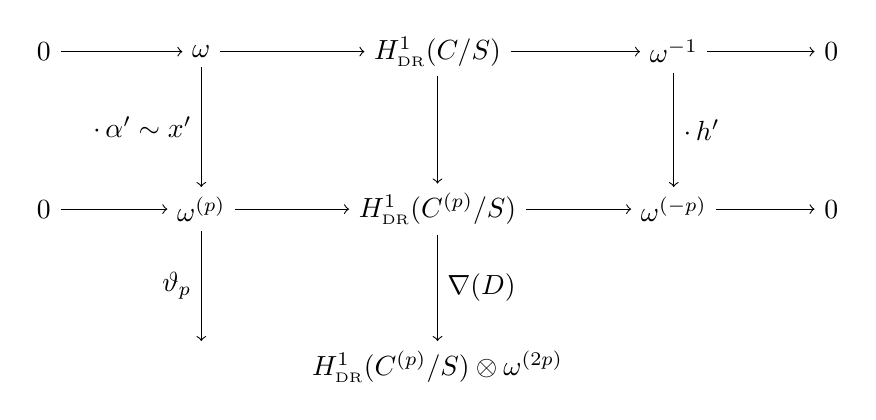
\begin{tikzpicture}
	\node (T1) at (0, 4) {$0$};
	\node (T2) at (2, 4) {$\omega$};
	\node (T3) at (5, 4) {$H_{\DR}^1(C/S)$};
	\node (T4) at (8, 4) {$\omega^{-1}$};
	\node (T5) at (10, 4) {$0$};
	\node (M1) at (0, 2) {$0$};
	\node (M2) at (2, 2) {$\omega^{(p)}$};
	\node (M3) at (5, 2) {$H_{\DR}^1(C^{(p)}/S)$};
	\node (M4) at (8, 2) {$\omega^{(-p)}$};
	\node (M5) at (10, 2) {$0$};
        \node (B2) at (2, 0.2) {$ $};
	\node (B3) at (5, 0) {$H_{\DR}^1(C^{(p)}/S) \otimes \omega^{(2 p)}$};
	\draw [->] (T1) -- (T2);
	\draw [->] (T2) -- (T3);
	\draw [->] (T3) -- (T4);
	\draw [->] (T4) -- (T5);
	\draw [->] (M1) -- (M2);
	\draw [->] (M2) -- (M3);
	\draw [->] (M3) -- (M4);
	\draw [->] (M4) -- (M5);
	\draw [->] (T2) -- node [left] {$\cdot \, \A' \sim x'$} (M2);
	\draw [->] (T3) -- (M3);
	\draw [->] (T4) -- node [right] {$\cdot \, h'$} (M4);
	\draw [->] (M2) -- node [left] {$\vartheta_p$} (B2);
	\draw [->] (M3) -- node [right] {$\nabla(D)$} (B3);
 \end{tikzpicture}
\end{center}

$\todo$ Look into more of \cite{padicprop} for a structural explanation of the appearance of Serre derivatives in homotopy-theoretic context.  



% \bibliographystyle{amsalpha}
% \bibliography{me}
% \end{document}

\vspace{.3in}
\renewcommand\refname{}
\newcommand{\AX}[1]{\href{http://arxiv.org/abs/#1}{arXiv:#1}}
\newcommand{\MRn}[2]{\href{http://www.ams.org/mathscinet-getitem?mr=#1}{MR#1#2}}
\wt{.}\vspace{-1.04in}
\begin{thebibliography}

\section*{\leftskip=-.44in References \vspace{.17in}}

\bibitem[Ahlgren2003]{Ahlgren}
Scott Ahlgren, \emph{The theta-operator and the divisors of modular forms on
  genus zero subgroups}, Math. Res. Lett. \textbf{10} (2003), no.~6,
  787--798. \MRn{2024734}{(2004m:11059)}

\bibitem[Ando1995]{Ando95}
Matthew Ando, \emph{Isogenies of formal group laws and power operations in the
  cohomology theories {$E\sb n$}}, Duke Math. J. \textbf{79} (1995), no.~2,
  423--485. \MRn{1344767}{(97a:55006)}

\bibitem[Apostol1990]{Apostol}
Tom~M. Apostol, \emph{Modular functions and {D}irichlet series in number
  theory}, second ed., Graduate Texts in Mathematics, vol.~41, Springer-Verlag,
  New York, 1990. \MRn{1027834}{(90j:11001)}

\bibitem[Atkin-Lehner1970]{AtkinLehner}
A.~O.~L. Atkin and J.~Lehner, \emph{Hecke operators on {$\Gamma \sb{0}(m)$}},
  Math. Ann. \textbf{185} (1970), 134--160. \MRn{0268123}{(42 \#3022)}

\bibitem[Bruinier-Kohnen-Ono2004]{BKO}
Jan~H. Bruinier, Winfried Kohnen, and Ken Ono, \emph{The arithmetic of the
  values of modular functions and the divisors of modular forms}, Compos. Math.
  \textbf{140} (2004), no.~3, 552--566. \MRn{2041768}{(2005h:11083)}

\bibitem[Choi2006]{Choi}
D.~Choi, \emph{On values of a modular form on {$\Gamma\sb 0(N)$}}, Acta Arith.
  \textbf{121} (2006), no.~4, 299--311. \MRn{2224397}{(2006m:11051)}

\bibitem[Deligne-Rapoport1973]{DR}
P.~Deligne and M.~Rapoport, \emph{Les sch\'emas de modules de courbes
  elliptiques}, Modular functions of one variable, {II} ({P}roc. {I}nternat.
  {S}ummer {S}chool, {U}niv. {A}ntwerp, {A}ntwerp, 1972), Springer, Berlin,
  1973, pp.~143--316. Lecture Notes in Math., Vol. 349. \MRn{0337993}{(49
  \#2762)}

\bibitem[Diamond-Shurman2005]{MF}
Fred Diamond and Jerry Shurman, \emph{A first course in modular forms},
  Graduate Texts in Mathematics, vol. 228, Springer-Verlag, New York, 2005.
  \MRn{2112196}{(2006f:11045)}

\bibitem[Kaneko-Zagier1998]{KanekoZagier}
M.~Kaneko and D.~Zagier, \emph{Supersingular {$j$}-invariants, hypergeometric
  series, and {A}tkin's orthogonal polynomials}, Computational perspectives on
  number theory ({C}hicago, {IL}, 1995), AMS/IP Stud. Adv. Math., vol.~7, Amer.
  Math. Soc., Providence, RI, 1998, pp.~97--126. \MRn{1486833}{(99b:11064)}

\bibitem[Katz1973]{padicprop}
Nicholas~M. Katz, \emph{{$p$}-adic properties of modular schemes and modular
  forms}, Modular functions of one variable, {III} ({P}roc. {I}nternat.
  {S}ummer {S}chool, {U}niv. {A}ntwerp, {A}ntwerp, 1972), Springer, Berlin,
  1973, pp.~69--190. Lecture Notes in Mathematics, Vol. 350. \MRn{0447119}{(56
  \#5434)}

\bibitem[Katz-Mazur1985]{KM}
Nicholas~M. Katz and Barry Mazur, \emph{Arithmetic moduli of elliptic curves},
  Annals of Mathematics Studies, vol. 108, Princeton University Press,
  Princeton, NJ, 1985. \MRn{772569}{(86i:11024)}

\bibitem[Kerner2008]{Kerner}
D.~Kerner, \emph{Enumeration of uni-singular algebraic hypersurfaces}, Proc.
  Lond. Math. Soc. (3) \textbf{96} (2008), no.~3, 623--668. \MRn{2407815}{(2009e:14088)}

\bibitem[Lubin1979]{can}
Jonathan Lubin, \emph{Canonical subgroups of formal groups}, Trans. Amer. Math.
  Soc. \textbf{251} (1979), 103--127. \MRn{531971}{(80j:14039)}

\bibitem[Milas-Mortenson-Ono2008]{MilasMortensonOno}
Antun Milas, Eric Mortenson, and Ken Ono, \emph{Number theoretic properties of
  {W}ronskians of {A}ndrews-{G}ordon series}, Int. J. Number Theory \textbf{4}
  (2008), no.~2, 323--337. \MRn{2404804}{(2009g:11054)}

\bibitem[Ono2004]{web}
Ken Ono, \emph{The web of modularity: arithmetic of the coefficients of modular
  forms and {$q$}-series}, CBMS Regional Conference Series in Mathematics, vol.
  102, Published for the Conference Board of the Mathematical Sciences,
  Washington, DC; by the American Mathematical Society, Providence, RI, 2004.
  \MRn{2020489}{(2005c:11053)}

\bibitem[Rezk2009]{cong}
Charles Rezk, \emph{The congruence criterion for power operations in {M}orava
  {$E$}-theory}, Homology, Homotopy Appl. \textbf{11} (2009), no.~2, 327--379.
  \MRn{2591924}{(2011e:55021)}

\bibitem[Silverman2009]{AEC}
Joseph~H. Silverman, \emph{The arithmetic of elliptic curves}, second ed.,
  Graduate Texts in Mathematics, vol. 106, Springer, Dordrecht, 2009.
  \MRn{2514094}{(2010i:11005)}

\bibitem[Strickland1997]{Str97}
Neil~P. Strickland, \emph{Finite subgroups of formal groups}, J. Pure Appl.
  Algebra \textbf{121} (1997), no.~2, 161--208. \MRn{1473889}{(98k:14065)}

\bibitem[Strickland1998]{Str98}
N.~P. Strickland, \emph{Morava {$E$}-theory of symmetric groups}, Topology
  \textbf{37} (1998), no.~4, 757--779. \MRn{1607736}{(99e:55008)}

\bibitem[Zhu2014]{p3}
Yifei Zhu, \emph{The power operation structure on {M}orava {$E$}-theory of
  height 2 at the prime 3}, Algebr. Geom. Topol. \textbf{14} (2014), no.~2,
  953--977. \MRn{3160608}{}

\bibitem[Zhu2015]{ho}
Yifei Zhu, \emph{The {H}ecke algebra action on {M}orava {$E$}-theory of height
  2}, available at \\ \href{http://www.math.northwestern.edu/~zyf/draft.pdf}
  {http://www.math.northwestern.edu/\textasciitilde zyf/draft.pdf}.

\end{thebibliography}



\end{document}